% Mitigating User Interface Latency Caused by Event Accumulation in an
% Online Video Editor Built on a Client-Server Architecture
% Copyright (C) 2012  Michael Chang
% based on
% uw-wkrpt-se.tex - An example work report that uses uw-wkrpt.cls
% Copyright (C) 2002,2003  Simon Law
% 
% This program is free software; you can redistribute it and/or modify
% it under the terms of the GNU General Public License as published by
% the Free Software Foundation; either version 2 of the License, or
% (at your option) any later version.
% 
% This program is distributed in the hope that it will be useful,
% but WITHOUT ANY WARRANTY; without even the implied warranty of
% MERCHANTABILITY or FITNESS FOR A PARTICULAR PURPOSE.  See the
% GNU General Public License for more details.
% 
% You should have received a copy of the GNU General Public License
% along with this program; if not, write to the Free Software
% Foundation, Inc., 59 Temple Place, Suite 330, Boston, MA  02111-1307  USA
%
%%%%%%%%%%%%%%%%%%%%%%%%%%%%%%%%%%%%%%%%%%%%%%%%%%%%%%%%%%%%%%%%%%%%%
%
% We begin by calling the workreport class which includes all the
% definitions for the macros we will use.
\documentclass[se,resubmit]{uw-wkrpt}

% LaTeX preamble: load some packages to add functionality
\usepackage{graphicx} % Include graphic importing

\usepackage[T1]{fontenc} % Better fonts
\usepackage{ae,aecompl}

\usepackage{indentfirst} % Indent first paragraph of each section

\usepackage[titletoc,title]{appendix} % Prefix appendix letters with `Appendix'

% For mathematical symbols in our pseudocode
\usepackage{amsmath}

% Use the algorithmicx package for pseudocode
\usepackage{algorithm}
\usepackage{algpseudocode}

% Use biblatex for references
\usepackage[style=ieee,sorting=none,dateabbrev=false,backend=biber]{biblatex}
\addbibresource{report.bib} % Specify the bibliography file

% This needs to be the last package loaded
\usepackage[pdftex]{hyperref} % Generate PDF links and bookmarks.
\hypersetup{
  bookmarks=true,
  bookmarksnumbered=true
}

% Now we will begin writing the document.
\begin{document}

%%%%%%%%%%%%%%%%%%%%%%%%%%%%%%%%%%%%%%%%%%%%%%%%%%%%%%%%%%%%%%%%%%%%%
%% IMPORTANT INFORMATION
%%%%%%%%%%%%%%%%%%%%%%%%%%%%%%%%%%%%%%%%%%%%%%%%%%%%%%%%%%%%%%%%%%%%%

%% First we, should create a title page.  This is done below:
% Fill in the title of your report.
\title{ Mitigating User Interface Latency Caused by Event Accumulation in an
Online Video Editor Built on a Client-Server Architecture }

% Fill in your name.
\author{Michael Chang}

% Fill in your student ID number.
\uwid{20332377}

% Fill in the name of the PNG file with your signature, or leave unchanged.
\signature{signature}

% Fill in your home address.
\address{30 Doncrest Rd.\\*
         Richmond Hill, ON\ \ L4B 1A2}

% Fill in your employer's name.
\employer{Google Inc.}

% Fill in your employer's city and province.
\employeraddress{Mountain View, CA}

% Fill in your school's name.
\school{University of Waterloo}

% Fill in your faculty name.
\faculty{Software Engineering}

% Fill in your student user ID
\userid{m9chang}

% Fill in your e-mail address.
\email{m9chang@uwaterloo.ca}

% Fill in your term.
\term{3A}

% Fill in your program.
\program{Software Engineering}

% Fill in the department chair's name.
\chair{Dr.\ A.\ Morton}

% Fill in the department chair's mailing address.
\chairaddress{Software Engineering\\*
              University of Waterloo\\*
	      Waterloo, ON\ \ N2L 3G1}

% If you are writing an "SE-confidential" report, uncomment the next line.
%\confidential{SE-confidential}

% If you want to specify the date, fill it in here.  If you comment out
% this line, today's date will be substituted.
\date{December 12, 2012}

% Now, we ask LaTeX to generate the title.
\maketitle

%%%%%%%%%%%%%%%%%%%%%%%%%%%%%%%%%%%%%%%%%%%%%%%%%%%%%%%%%%%%%%%%%%%%%
%% FRONT MATTER
%%%%%%%%%%%%%%%%%%%%%%%%%%%%%%%%%%%%%%%%%%%%%%%%%%%%%%%%%%%%%%%%%%%%%
%% \frontmatter will make the \section commands ignore their numbering,
%% it will also use roman page numbers.
\frontmatter

% After this, we must create a letter of submission.
\begin{letter}
I have just completed my fourth work term, following my \theterm{} term.  Please
find enclosed my third work term report entitled: ``\thetitle'' for YouTube,
LLC, a subsidiary of \theemployer.  My manager was Bob Glickstein, and our team
was primarily involved with building tools for video creators and content
curators.

This report focuses on the handling of input events in the video enhancement
tool on YouTube. This problem is similar to one that I encountered on my work
term, but has been modified to protect proprietary design decisions.

I wish to thank B. Glickstein and R. Doshi for their advice on the technical
content of this report. I also wish to thank C. Kleynhans and M. Yee for their
advice on choosing a word processing environment to write this report. In
addition, I wish to thank W. Chang for proofreading this report. Finally, I wish
to thank A. Mortezaei for providing feedback on the initial submission of this
report.
% Note that I do not need to type out the boilerplate confirmation,
% nor do I need to write a signature block.  This is generated for me.
% We are now finished with the letter.
\end{letter}

% We continue with required sections, such as the Executive Summary.
\section{Executive Summary}
AudioSwap is one of the video enhancement features available to video creators
on YouTube. It allows video creators to select a song from a library of over
100,000 songs that YouTube has licensed. The initial implemention of AudioSwap
only allowed users to place the audio at the beginning of their video, and to
use the song in its entirety. One of the major accomplishments of my work term
was to implement user interface changes which allow video creators to position
and trim tracks they've placed over their videos using AudioSwap.

This document describes issues which arose when these changes were first
publicly deployed. It also describes some ways those issues could be mitigated,
and uses the multi-criteria decision making methdology to rank these mitigation
strategies. Finally, it discusses these issues in the context of the material in
CS 349 - User Interfaces, which is a core course in the Software Engineering
curriculum, and presents some general considerations for adapting the lessons
learned from the issues presented to future software projects.

% Next, we need to make a Table of Contents, List of Figures and 
% List of Tables.  You will most likely need to run LaTeX twice to
% get these correct.  The first pass for LaTeX to figure out the
% labels, and the second pass to put in the right references.
\tableofcontents
\listoffigures
\listoftables

%%%%%%%%%%%%%%%%%%%%%%%%%%%%%%%%%%%%%%%%%%%%%%%%%%%%%%%%%%%%%%%%%%%%%
%% REPORT BODY
%%%%%%%%%%%%%%%%%%%%%%%%%%%%%%%%%%%%%%%%%%%%%%%%%%%%%%%%%%%%%%%%%%%%%
%% \main will make the \section commands numbered again,
%% it will also use arabic page numbers.
\mainmatter

% You must have an Introduction
\section{Introduction}\label{sec:intro}
YouTube provides a web-based tool that allows users to perform minor
enhancements to their videos without installing additional software on their
computer.

The enhancement tool is comprised of two parts: client-side code and preview
servers. The client-side code is primarily written in JavaScript, and runs in
users' web browsers. The preview servers run on proprietary Google
infrastructure.

When a user modifies a video with the tool, the client-side code generates a
computer-readable description of the changes made to the video called an edit
list. The client-side code then sends the edit list to the preview server. The
preview server uses the edit list and the user's original video (which has
already been uploaded to YouTube) to generate a low-fidelity version of the
video. It returns the location of the low-fidelity preview video to the
client-side code, which then displays the preview video to the user.

\section{Problem Statement}\label{sec:problem}
A large number of UI events may be generated when the user positions or trims an
audio clip on the enhance page. When a large number of events occur, the user
experiences a large delay before seeing a preview that corresponds with their
most recent change.

In order to protect proprietary design decisions, it is assumed that a user
interaction generates 150 events over five seconds at a constant rate of 30
events per second. It is also assumed that requests will be processed one at a
time.\footnote{According to \cite{ref:http}, HTTP user agents should limit
themselves to two concurrent requests. It can be seen in \cite{ref:b423377} that
many browsers use more (say, four or six). However, this is omitted from the
simulations for simplicity.} Finally, it is assumed that a server response will
take 600 ms.\footnote{The calculation to determine this figure is noted in
\ref{app:calculating}.}

A simulation of the request queue length for the first 100 seconds after the
start of the interaction is shown in \ref{fig:sim-orig}.

\begin{figure}
  \centering
  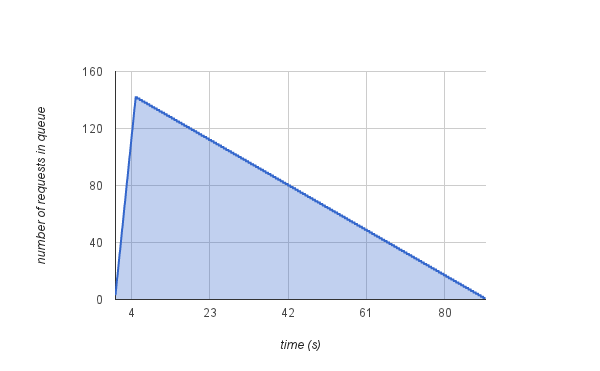
\includegraphics{sim-orig}
  \caption{Simulated Request Queue Length (Original Implementation).}
  \label{fig:sim-orig}
\end{figure}

% You must have either an Analysis or a Synthesis section.
\section{Analysis}

First, the multi-criteria decision making (MCDM) methodology (see
\ref{tbl:mcdm}) is used to evaluate a few possible solutions. Higher scores are
better. Possible solutions were generated through brainstorming.  The
methodology used to select the criteria and weights is outside of the scope of
this report.
% FIXME No they're not, apparently!

The results of \ref{tbl:mcdm} indicate that sending one edit list to the
preview server every $\Delta t$ is the best solution. A number of simulations was
performed to determine the best value of $\Delta t$. A sample of these
simulations is shown below in \ref{fig:sim-300ms}, \ref{fig:sim-600ms}, and \ref{fig:sim-1000ms}. Of the simulations performed, the value
$\Delta t=600 ms$ provided the most frequent preview updates to the user while
maintaining a bounded request queue size, and thus it is recommended that the
implementation be changed to send an edit list to the preview server every 600
ms.

% Here is a table.  You MUST cite the table in the text before it appears
% in the document.
\begin{table}
  \caption{Multi-Criteria Decision Making Results.}
  \label{tbl:mcdm}
  \centering
  \begin{tabular}{|p{2.0cm}|p{1.0cm}|p{1.25cm}|p{1.25cm}|p{1.25cm}|p{1.25cm}|
                                     p{1.25cm}|p{1.25cm}|p{1.25cm}|p{1.25cm}|}
    \hline
    \textbf{Criteria} &
    \textbf{Wt.} &
    \multicolumn{2}{|p{2.5cm}|}{\textbf{Send only the last edit list to preview
    server.}} &
    \multicolumn{2}{|p{2.5cm}|}{\textbf{Send one edit list to the preview
    server every $\Delta t$.}} &
    \multicolumn{2}{|p{2.5cm}|}{\textbf{Increase number of concurrent
    connections.}} &
    \multicolumn{2}{|p{2.5cm}|}{\textbf{Do nothing.}} \\
    \hline\hline
    Minimizes Time to Receipt of Last Response &
       4 &  4 & 16 &  3 & 12 &  2 &  8 &  1 &  4 \\
    \hline
    Minimizes Server Resources Used &
       2 &  4 &  8 &  3 &  6 &  1 &  2 &  1 &  2 \\
    \hline
    Displays Feedback to User During Interaction &
       3 &  1 &  3 &  4 & 12 &  3 &  9 &  2 &  6 \\
    \hline
    Does Not Require Client Configuration &
       5 &  4 & 20 &  4 & 20 &  1 &  5 &  4 & 20 \\
    \hline
    Minimizes Developer Effort &
       1 &  2 &  2 &  2 &  2 &  3 &  3 &  4 &  4 \\
    \hline
    \hline
    \textbf{Total} &
      &
      \multicolumn{2}{|r|}{\textbf{49}} &
      \multicolumn{2}{|r|}{\textbf{52}} &
      \multicolumn{2}{|r|}{\textbf{27}} &
      \multicolumn{2}{|r|}{\textbf{36}} \\
    \hline
  \end{tabular}
\end{table}

\begin{figure}
  \centering
  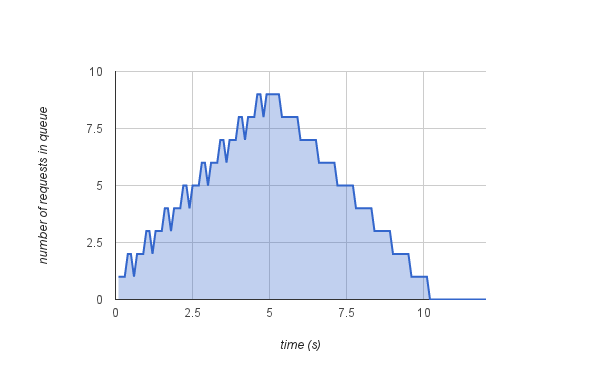
\includegraphics{sim-300ms}
  \caption{Simulated Request Queue Length (300ms delay).}
  \label{fig:sim-300ms}
\end{figure}

\begin{figure}
  \centering
  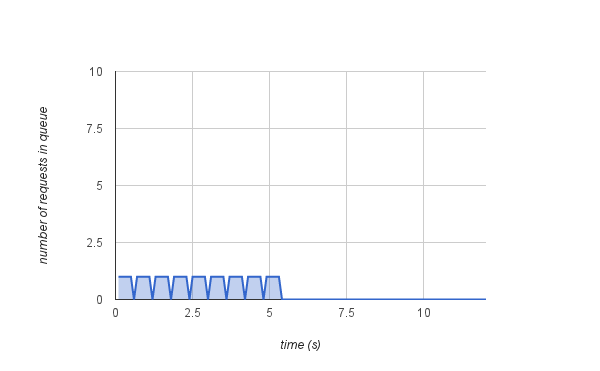
\includegraphics{sim-600ms}
  \caption{Simulated Request Queue Length (600ms delay).}
  \label{fig:sim-600ms}
\end{figure}

\begin{figure}
  \centering
  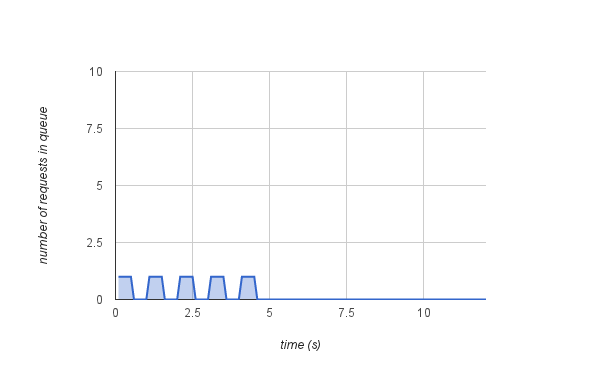
\includegraphics{sim-1000ms}
  \caption{Simulated Request Queue Length (1000ms delay).}
  \label{fig:sim-1000ms}
\end{figure}

% You must have a Conclusions section
\section{Conclusions}
It is proposed that the edit lists be sent to the preview server at most once
every 600 ms. This provides a bound on the size of the number of requests in the
queue. (Only one request will be processing at any given time.) This gives us a
bound on the time between a given user interaction and when the preview is
displayed to the user. This also reduces the total number of preview requests
sent to the preview server, which results in a corresponding reduction in CPU
and bandwidth usage on the server.

% You must have a Recommendations section
\section{Recommendations}
Sending edit lists to the preview server should be rate-limited to at most once
every 600 ms.

%%%%%%%%%%%%%%%%%%%%%%%%%%%%%%%%%%%%%%%%%%%%%%%%%%%%%%%%%%%%%%%%%%%%%
%% BACK MATTER
%%%%%%%%%%%%%%%%%%%%%%%%%%%%%%%%%%%%%%%%%%%%%%%%%%%%%%%%%%%%%%%%%%%%%
%% \backmatter will make the \section commands ignore their numbering,
\backmatter

% Here, we insert a References section, which will be formatted properly.
% The list of works you have referenced should be specified in the preamble.
% In this template, the file is uw-wkrpt-bib.bib.
%
% Note, you will need to process the document in a certain order.  First,
% run LaTeX.  The % first pass will allow LaTeX to build a list of 
% references, it may % emit warning messages such as:
%   LaTeX Warning: Reference `app:gnugpl' on page 4 undefined on input line 277.
%   LaTeX Warning: There were undefined references.
% This is normal.  Now you run BiBTeX in order to generate the proper
% layout for the references.  After this, you run LaTeX once more.
\printbibliography[heading=bibintoc]

\section{Acknowledgements}
% This section shall acknowledge the people who helped with the writing 
% of the work report. This would include anyone who was interviewed, 
% anyone who proofread the report, or anyone whose files were used in 
% the writing of the report.
I would like to thank J. Doe for proofreading this report.

I used the \textsf{uw-wkrpt} document class written by Simon Law to 
typeset it.

%%%%%%%%%%%%%%%%%%%%%%%%%%%%%%%%%%%%%%%%%%%%%%%%%%%%%%%%%%%%%%%%%%%%%
%% APPENDICES
%%%%%%%%%%%%%%%%%%%%%%%%%%%%%%%%%%%%%%%%%%%%%%%%%%%%%%%%%%%%%%%%%%%%%
%% \appendix will reset \section numbers and turn them into letters.
%%
%% Don't forget to refer to all your appendices in the main report.
\appendix
\begin{appendices}

\section{Calculating Simulated Server Response Time}\label{app:calculating}
The simulated server response time is comprised by summing multiple factors, as
noted below.

\subsection{Round Trip Time}
Round-trip travel times between three locations in North America and youtube.com
were sampled.

\begin{table}
  \caption{Round Trip Time.}
  \label{tbl:rtt}
  \centering
  \begin{tabular}{|p{2.0cm}|p{2.0cm}|p{2.0cm}|p{2.0cm}|p{2.0cm}|p{2.0cm}|
                   p{2.0cm}|}
    \hline
    \textbf{Location} &
    \textbf{Trial 1} &
    \textbf{Trial 2} &
    \textbf{Trial 3} &
    \textbf{Trial 4} &
    \textbf{Mean} &
    \textbf{Sample StDev} \\
    \hline
    \hline
    Richmond Hill, Ontario &
      7.77 & 7.16 & 6.85 & 7.44 & 7.305 & 0.393 \\
    \hline
    Waterloo, Ontario &
      6.16 & 6.09 & 6.28 & 6.12 & 6.163 & 0.083 \\
    \hline
    Fremont, California &
      1.18 & 1.30 & 1.18 & 1.28 & 1.235 & 0.064 \\
    \hline
    \hline
    \multicolumn{5}{|p{10.0cm}|}{\textbf{Average}} &
      4.901 & 2.759 \\
    \hline
  \end{tabular}
\end{table}

\subsection{Encoding Time}
To protect proprietary design decisions, assume it takes 2000 ms to encode 1000
s (~= 16 minutes) of audio. (Video encoding time is ignored; since the control
only alters the audio track, we assume that existing video encodes can be reused
and multiplexed into the result upon being sent to the client.) We take the
average of the durations of top featured tracks in the audio enhancement page to
get an approximate audio duration of 4 minutes, 53.125 seconds. Based on our
assumption, this would take 587 ms to encode.

\subsection{Wi-Fi}
The use of a wireless network standard such as 802.11n may introduce additional
latency in the HTTP request. The amount of this latency varies depending on many
factors, and could be the subject of its own report. It is assumed that the user
is using a wired connection for the purposes of this report. It should be noted
that the final implementation may need further adjustment to compensate for the
extra latency that users of these networks will encounter.

\subsection{Other Factors}
It is assumed that other tasks like multiplexing the audio and video streams on
the preview server, and server-side parsing of the edit list are almost
negligible. The duration of these tasks should be dwarfed by the time taken to
encode the audio on the preview server. We add 8 ms of latency to account for
these other factors.

\end{appendices}
\end{document}
